
%% This is file `sample-acmsmall.tex',
%% generated with the docstrip utility.
%%
%% The original source files were:
%%
%% samples.dtx  (with options: `acmsmall')
%% 
%% IMPORTANT NOTICE:
%% 
%% For the copyright see the source file.
%% 
%% Any modified versions of this file must be renamed
%% with new filenames distinct from sample-acmsmall.tex.
%% 
%% For distribution of the original source see the terms
%% for copying and modification in the file samples.dtx.
%% 
%% This generated file may be distributed as long as the
%% original source files, as listed above, are part of the
%% same distribution. (The sources need not necessarily be
%% in the same archive or directory.)
%%
%% The first command in your LaTeX source must be the \documentclass command.
\documentclass[sigplan,anonymous,review]{acmart}
\usepackage[switch]{lineno}
\usepackage{booktabs}
\usepackage{listings}
\usepackage{tcolorbox}
\usepackage{tikz}
\usepackage{tkz-graph}
\usepackage{stmaryrd}
\usepackage{amsmath}

% \lstset{basicstyle=\ttfamily}
\usetikzlibrary{shapes.geometric, arrows}

\tikzstyle{startstop} = [rectangle, rounded corners, minimum width=3cm, minimum height=1cm,text centered, draw=black, fill=red!30]
\tikzstyle{process} = [rectangle, minimum width=3cm, text width=0.3*\columnwidth, minimum height=1cm, text centered, draw=black, fill=orange!30]
\tikzstyle{decision} = [diamond, minimum width=3cm, minimum height=1cm, text centered, draw=black, fill=green!30]
\tikzstyle{arrow} = [thick,->,>=stealth]


% \renewcommand{\linenumberfont}{\color{blue}}

% \renewcommand\linenumberfont{\normalfont\tiny\sffamily\color{red}}

\lstset{language=haskell, deletekeywords={abs},basicstyle=\ttfamily}

\newcommand{\expr}[1]{(#1)} % Expression quasiquote
\newcommand{\rarr}{\rightarrow}
\newcommand{\Rarr}{\Rightarrow}
\newcommand{\rewrites}{\Longrightarrow}

% TODO: Use these:
\newcommand{\exprt}[1]{\expr{\ttt{#1}}}
\newcommand{\tdots}{\ttt{...}}
\newcommand{\exprdots}{\expr{\tdots}}

\newcommand{\typeeq}{\raise.17ex\hbox{$\scriptstyle\mathtt{\sim}$}\,\;}

\newcommand{\ttt}{\texttt}

\newcommand{\showtodos}{}  % Comment out to hide todos

\newenvironment{todo}
  {\ifthenelse{\isundefined{\showtodos}}{\comment}{\begin{tcolorbox}
    \textbf{TODO}:}}
  {\ifthenelse{\isundefined{\showtodos}}{\endcomment}{\end{tcolorbox}}
  }
\newenvironment{todont}
               {\comment}
               {\endcomment}
  
% \newenvironment<>{todo}[1][]{
%     \setbeamercolor{block body example}{fg=black,bg=blue}
%     \setbeamercolor{block title example}{fg=white,bg=red!75!black}
%     \setbeamertemplate{blocks}[rounded][shadow=false]
%   \begin{todo}[]}{\end{todo}
% }

%%
%% \BibTeX command to typeset BibTeX logo in the docs
\AtBeginDocument{%
  \providecommand\BibTeX{{%
    \normalfont B\kern-0.5em{\scshape i\kern-0.25em b}\kern-0.8em\TeX}}}

%% Rights management information.  This information is sent to you
%% when you complete the rights form.  These commands have SAMPLE
%% values in them; it is your responsibility as an author to replace
%% the commands and values with those provided to you when you
%% complete the rights form.

\setcopyright{acmcopyright}
\copyrightyear{2020}
\acmYear{2020}
\acmDOI{XX.XXXX/XXXXXXX}


%% These commands are for a PROCEEDINGS abstract or paper.

\acmConference[GPCE '20]{GPCE '20: Proceedings of the 13th
  ACM SIGPLAN International Symposium on Haskell}{November 15 -- 20, 2020}{Chicago, Illinois, United States}
\acmBooktitle{Proceedings of the 19th ACM SIGPLAN International
Conference on Generative Programming: Concepts and Experiences (GPCE '20)
  November 15 -- 20, 2020, Chicago, Illinois, United States}
\acmPrice{15.00}
\acmISBN{XXX-X-XXXX-XXXX-X/XX/XX}


\citestyle{acmauthoryear}

%%
%% Submission ID.
%% Use this when submitting an article to a sponsored event. You'll
%% receive a unique submission ID from the organizers
%% of the event, and this ID should be used as the parameter to this command.
%%\acmSubmissionID{123-A56-BU3}

%%
%% The majority of ACM publications use numbered citations and
%% references.  The command \citestyle{authoryear} switches to the
%% "author year" style.
%%
%% If you are preparing content for an event
%% sponsored by ACM SIGGRAPH, you must use the "author year" style of
%% citations and references.
%% Uncommenting
%% the next command will enable that style.
%%\citestyle{acmauthoryear}

%%
%% end of the preamble, start of the body of the document source.

\begin{document}

%%
%% The "title" command has an optional parameter,
%% allowing the author to define a "short title" to be used in page headers.
\title{On Adding Pattern Matching to Haskell-based
  Deeply Embedded Domain Specific Languages}

%%
%% The "author" command and its associated commands are used to define
%% the authors and their affiliations.
%% Of note is the shared affiliation of the first two authors, and the
%% "authornote" and "authornotemark" commands
%% used to denote shared contribution to the research.
\author{David Young}
\email{d063y800@ku.edu}

% \authornote{Both authors contributed equally to this research.}
% \email{trovato@corporation.com}
% \orcid{1234-5678-9012}

\author{Mark Grebe}
\email{grebe@ucmo.edu}

\author{Andrew Gill}
\email{andygill@ku.edu}

%%
%% By default, the full list of authors will be used in the page
%% headers. Often, this list is too long, and will overlap
%% other information printed in the page headers. This command allows
%% the author to define a more concise list
%% of authors' names for this purpose.
% \renewcommand{\shortauthors}{Trovato and Tobin, et al.}
\renewcommand{\shortauthors}{Young, Grebe and Gill}

%%
%% The abstract is a short summary of the work to be presented in the
%% article.
\begin{abstract}
% Say what problem is
  Capturing control flow is the Achilles heel of Haskell-based
  deeply embedded domain specific languages.
  Rather than use
  the builtin control flow mechanisms, artificial control flow combinators
  are used instead.
% Say why it is an interesting problem
  However, capturing traditional control flow in an deeply embedded domain specific language
  would support the writing of programs in a natural style by allowing the programmer to use the
  constructs that are already builtin to the base language, such as pattern
  matching and recursion.
% Say what our solution achieves
  In this paper, we expand the capabilities of
  Haskell-based deep embeddings with a compiler extension
  for reifying conditionals and pattern matching.
% Here is why the world will be a better place
  With this new support, the Haskell that we capture for expressing
  deeply embedded domain specific languages can be cleaner, Haskell-idiomatic,
  and more declarative in nature.

\end{abstract}

\begin{CCSXML}
<ccs2012>
   <concept>
       <concept_id>10011007.10011006.10011041.10011046</concept_id>
       <concept_desc>Software and its engineering~Translator writing systems and compiler generators</concept_desc>
       <concept_significance>300</concept_significance>
       </concept>
   <concept>
       <concept_id>10011007.10011006.10011041.10011047</concept_id>
       <concept_desc>Software and its engineering~Source code generation</concept_desc>
       <concept_significance>300</concept_significance>
       </concept>
   <concept>
       <concept_id>10011007.10011006.10011050.10011017</concept_id>
       <concept_desc>Software and its engineering~Domain specific languages</concept_desc>
       <concept_significance>500</concept_significance>
       </concept>
 </ccs2012>
\end{CCSXML}

\ccsdesc[300]{Software and its engineering~Translator writing systems and compiler generators}
\ccsdesc[300]{Software and its engineering~Source code generation}
\ccsdesc[500]{Software and its engineering~Domain specific languages}


% \begin{CCSXML}
% <ccs2012>
%    <concept>
%        <concept_id>10011007.10011006.10011050.10011017</concept_id>
%        <concept_desc>Software and its engineering~Domain specific languages</concept_desc>
%        <concept_significance>500</concept_significance>
%        </concept>
%  </ccs2012>
% \end{CCSXML}

% \ccsdesc[500]{Software and its engineering~Domain specific languages}

% \keywords{domain specific languages}

%%
%% The code below is generated by the tool at http://dl.acm.org/ccs.cfm.
%% Please copy and paste the code instead of the example below.
%%
% \begin{CCSXML}
% <ccs2012>
%  <concept>
%   <concept_id>10010520.10010553.10010562</concept_id>
%   <concept_desc>Computer systems organization~Embedded systems</concept_desc>
%   <concept_significance>500</concept_significance>
%  </concept>
%  <concept>
%   <concept_id>10010520.10010575.10010755</concept_id>
%   <concept_desc>Computer systems organization~Redundancy</concept_desc>
%   <concept_significance>300</concept_significance>
%  </concept>
%  <concept>
%   <concept_id>10010520.10010553.10010554</concept_id>
%   <concept_desc>Computer systems organization~Robotics</concept_desc>
%   <concept_significance>100</concept_significance>
%  </concept>
%  <concept>
%   <concept_id>10003033.10003083.10003095</concept_id>
%   <concept_desc>Networks~Network reliability</concept_desc>
%   <concept_significance>100</concept_significance>
%  </concept>
% </ccs2012>
% \end{CCSXML}

% \ccsdesc[500]{Computer systems organization~Embedded systems}
% \ccsdesc[300]{Computer systems organization~Redundancy}
% \ccsdesc{Computer systems organization~Robotics}
% \ccsdesc[100]{Networks~Network reliability}

%%
%% Keywords. The author(s) should pick words that accurately describe
%% the work being presented. Separate the keywords with commas.
% \keywords{datasets, neural networks, gaze detection, text tagging}


%%
%% This command processes the author and affiliation and title
%% information and builds the first part of the formatted document.
\maketitle

\section{Introduction}

Embedded domain specific languages (EDSLs) have long been an effective
technique for constructing reusable tools for working in a variety of
different problem domains. Haskell is a language which is particularly
well-suited to EDSLs due to its lazy evaluation, first-class functions and
lexical closures.

Despite these advantages Haskell provides for creating EDSLs, there are a few
constructs for which representations have proven illusive. One prominent example
is that of a \ttt{case} expression. Pattern matching is a convenient way to
implement control flow structures and to inspect data structures, so it is
frequently a desirable feature for many EDSLs.

Additionally, lambdas can also be difficult to implement in EDSLs. A major reason
for this is that control flow constructs which are typically \textit{outside} the EDSL,
such as pattern matching and tail recursion, can make it challenging to "look inside"
the lambda. When these control structures are reified within the EDSL, it is
easier to also reify lambdas using the dummy argument technique described in~\cite{Elliott:03:CompileDSEL-JFP}.

% \begin{todo}
%   Maybe add brief summary of relationship to lambdas?
% \end{todo}

The following contributions are made by this paper:

\begin{itemize}
  \item A representation of pattern matching in a Haskell EDSL (Section~\ref{sec:PatRep})
  \item A representation of lambdas (Section~\ref{sec:LamRep}) in the EDSL, taking advantage of
  the fact that both pattern matching and tail recursion are already captured in
  the EDSL.
\item A GHC Core plugin which transforms a subset of standard Haskell code
  into this EDSL for pattern matching, extended with tail recursion,
  lambdas and primitive operations (Section~\ref{sec:CorePlugin})
\item An implementation of a interpreter for the "standard" semantics of the EDSL (Section~\ref{sec:StdSemantics}).
\item An outline of a C backend for this EDSL (Section~\ref{sec:CBackend}).
\end{itemize}

Readers who are primarily interested only in the encoding of pattern matching itself can direct
most of their attention to Sections~\ref{sec:ADTRep},~\ref{sec:PatRep} and~\ref{sec:StdSemantics}. Most of the technical aspects of
the transformation performed by the Core plugin are described in Section~\ref{sec:CorePlugin}.

\subsection{Motivation}

\begin{todont}
  Expand?
\end{todont}

A major benefit of the Haskell language is that it is frequently possible derive
a Haskell implementation from a specification, either partially or fully.
Examples of this technique include the work in \cite{Elliott-2018-ad-icfp} as
well as the work in \cite{Elliott2019-convolution-extended}.  When it is not
possible to fully derive an implementation from a specification, it is often
easier to check a Haskell implementation against a specification than it is in
many imperative languages due, in part, to the management of side effects in
Haskell. This is more difficult to do using an imperative language such as C, as
they provide no restrictions on where side effects can occur.

\newpage
Haskell EDSLs that support powerful language features like pattern matching
allow these advantages to be brought to problem domains where it is currently
either difficult or impossible to use a language that has these benefits.

\begin{todont}
  % Cite examples where Haskell implementations have been derived specifications.  Conal Elliott's latest two papers (as of May 2020), \cite{Elliott-2018-ad-icfp} and \cite{Elliott2019-convolution-extended}, would be good examples of this. (This is now cited)

  A paper which describes a Haskell implementation derived from an operational
  semantics would also be a good example.
\end{todont}

\subsection{Overview}
\label{sec:Overview}

In this EDSL, the type representing values in the expression language is \ttt{E
t} and there are two basic functions which translate values to and from this
expression language with the following type signatures (omitting type class
constraints for the moment):

\begin{lstlisting}
rep :: a -> E a
abs :: E a -> a
\end{lstlisting}

Additionally, the following functions mark the parts of the code which the Core
plugin will target:

\begin{lstlisting}
internalize :: E a -> a
externalize :: a -> E a
\end{lstlisting}

The \ttt{E} type is the type of expressions in the EDSL.  In this paper, the
data constructors of this type will be described incrementally as they
are needed.

\subsection{Translation Example}

% \begin{todo}
%   Does it make sense for this to be a subsection of the intro?
% \end{todo}

In the example below, the Core plugin transforms \ttt{example} into \ttt{example'}:
\begin{lstlisting}[deletekeywords={Ord}]
import Data.Char (ord)

x :: Either Char Int
x = Left 'a'

example :: Int
example =
  internalize (externalize
    (case x of
      Left  c -> ord c
      Right i -> i))

example' :: Int
example' =
  abs (CaseExp
        (LeftExp 'a')
        (SumMatchExp (OneProdMatch
                       (Lam 1
                         (Ord (Var 1))))
                     (OneSumMatch
                       (OneProdMatch
                         (Lam 2
                           (Var 2)))))
\end{lstlisting}

\section{Representing Algebraic Datatypes}
\label{sec:ADTRep}

% \begin{todo}
%   Look into \ttt{generic-sop} and compare then cite corresponding paper.
% \end{todo}

Briefly, a algebraic type \ttt{T} with an automatically generated \ttt{ERep}
instance is given a representation in terms of \ttt{Either}, \ttt{(,)}, \ttt{()}
and \ttt{Void}.  This "standardized" type representation is given by \ttt{ERepTy
T}. \ttt{ERepTy} is an type family associated to the type class \ttt{ERep}. This
type will be called the \textit{canonical type} of \ttt{T}.

Only the "outermost" type will be deconstructed into these fundamental building
blocks, and further deconstruction can take place on these pieces later on. For
example, consider this type:

\begin{lstlisting}
data ComplexPair where
  ComplexPair :: Complex Double
                 -> Complex Double
                 -> ComplexPair
  deriving (Generic, Show)

instance ERep ComplexPair
\end{lstlisting}

Note that the instance definition is automatically generated from the
\ttt{Generic} instance.

Given this code, \ttt{ERepTy ComplexPair \typeeq (Complex Double, Complex Double)}. Here
is an example that demonstrates why this is more useful than if it \textit{fully} deconstructed
each type into \ttt{Either}, \ttt{(,)} and \ttt{()}:

\begin{lstlisting}
sumComplexPair ::
  ComplexPair -> Complex Double
sumComplexPair p =
  internalize (externalize
    (case p of
      ComplexPair a b -> a + b))
\end{lstlisting}

If \ttt{ERepTy ComplexPair} were fully deconstructed into \ttt{((Double, Double),
(Double, Double))}, we would need a \ttt{Num} instance for \ttt{(Double,
Double)}.  What we really want is to use the fact that a \ttt{Num} instance
already exists for \ttt{Complex Double}. This is exactly what preserving this
type information allows us to do. We can later use this preserved type
information in backends, through the corresponding \ttt{Typeable} instances (for
instance, to provide special support for arithmetic on complex numbers).

It is important to note that we are still able to further deconstruct this type
with further pattern matches, since \ttt{ERepTy (Complex Double) \typeeq (Double, Double)}:

\begin{lstlisting}
realSum :: ComplexPair -> Double
realSum p =
  internalize (externalize
    (case p of
      ComplexPair a b -> case a of
          a_real :+ _ -> case b of
              b_real :+ _ ->
                a_real + b_real))
\end{lstlisting}

The above pattern matches could also be written as a single nested pattern
match. Both forms compile down to the same Core representation.

An additional benefit of this is that recursive types require no special handling. For
example, consider:

\begin{lstlisting}
data IntList = Nil | Cons Int IntList
  deriving (Generic, Show)

instance ERep IntList
\end{lstlisting}

Note that \ttt{ERepTy IntList \typeeq Either () (Int, IntList)}. If \ttt{ERepTy}
attempted to "fully deconstruct" \ttt{IntList}, it would send the compiler
into an infinite loop.

This allows us to implement functions on such recursive types:

\begin{lstlisting}
isEmpty :: IntList -> Bool
isEmpty t =
  internalize (externalize
    (case t of
      Nil -> True
      Cons x xs -> False))

intListSum :: (Int, IntList) -> Int
intListSum p =
  internalize (externalize
    (case p of
       (acc, t) ->
         case t of
           Nil -> acc
           Cons x xs ->
             intListSum
               (x+acc, xs)))
\end{lstlisting}

\subsection{\ttt{E}, \ttt{ERep}, \ttt{ERepTy}}

There are three interconnected foundational parts: \ttt{E}, \ttt{ERep} and
\ttt{ERepTy}. \ttt{E} is the deep embedding of the EDSL (a GADT that encodes
expressions in the DSL language). \ttt{ERep} is a type class which represents
all Haskell types which can be represented in the DSL. \ttt{ERepTy} is a type
family associated to the \ttt{ERep} type class, which represents a "canonical form"
of the given type. This canonical form can be immediately constructed in the EDSL.
Canonical form types crucially include \ttt{Either} and \ttt{(,)}, which
allow all combinations of basic sum types and product types to be encoded, in the
manner described at the beginning of Section~\ref{sec:ADTRep}.

With GHC Generics, any data type \ttt{T} with a \ttt{Generic} instance has a
corresponding \ttt{Rep T} type, which gives a generic representation of \ttt{T}.
Conversion between values of this type and values of the original type \ttt{T} is
given by the functions \ttt{to} and \ttt{from}. The generic representation \ttt{Rep T}
can be traversed by functions which operate solely on the structure of the data type.
This generic representation contains additional metadata which we do not need.
However, we can automatically generate a \ttt{ERep} instance for any type which
has a \ttt{Generic} instance.

As \ttt{Generic} instances are automatically generated, this provides a simple mechanism
to automaticly generate \ttt{ERep} instances.


This information is brought into the \ttt{E} type via the constructor
\ttt{ConstructRep}. The \ttt{E} also contains constructors representing \ttt{Either}
and \ttt{(,)} values:

\begin{lstlisting}
data E t where
  ...
  ConstructRep ::
    (Typeable a, ERep a)
    => E (ERepTy a) -> E a

  LeftExp :: E a -> E (Either a b)
  RightExp :: E b -> E (Either a b)

  PairExp :: E a -> E b -> E (a, b)
  ...
\end{lstlisting}

\ttt{ERep} and \ttt{ERepTy} provide an interface for transferring values between the EDSL
expression language and the source Haskell language:

\begin{lstlisting}
class Typeable t => ERep t where
  type ERepTy t

  construct :: t -> E (ERepTy t)
  rep :: t -> E t

  default rep ::
    (ERep (ERepTy t))
    => t -> E t
  rep x = ConstructRep (construct x)
  {-# INLINABLE rep #-}

  unrep' :: ERepTy t -> t
  rep' :: t -> ERepTy t
\end{lstlisting}

The key algebraic instances mentioned before are as follows:

\begin{lstlisting}
instance (ERep a, ERep b)
  => ERep (Either a b) where

  type ERepTy (Either a b) = Either a b

  rep (Left x)  = LeftExp (rep x)
  rep (Right y) = RightExp (rep y)
  unrep' = id
  rep'   = id

instance (ERep a, ERep b)
  => ERep (a, b) where

  type ERepTy (a, b) = (a, b)

  rep (x, y) = PairExp (rep x) (rep y)
  unrep' = id
  rep'   = id
\end{lstlisting}


\section{Representing pattern matches}
\label{sec:PatRep}

Within the \ttt{E} expression language, a pattern match is represented by the
\ttt{CaseExp} constructor:

\begin{lstlisting}
data E t where
  ...
  CaseExp ::
    (ERep t,
     ERepTy (ERepTy t) ~ ERepTy t)
      => ERep t
         -> E (SumMatch (ERepTy t) r)
         -> E r
  ...
\end{lstlisting}

The equality constraint ensures that a canonical type is its own canonical type.

% \begin{todo}
%   Should we make a synonym for this constraint since it is used in
% multiple places? Like this:
% \begin{lstlisting}
% type CanonicalIsIdem t =
%   ERepTy (ERepTy t) ~ ERepTy t
% \end{lstlisting}
% \end{todo}

(The above code block is a slight simplification of the actual implementation,
which has an additional type variable which is used at an "intermediate" point.
The expanded form is in place to simplify the Core transformation.)

The type \ttt{SumMatch} is defined as

\begin{lstlisting}
newtype SumMatch a b =
  MkSumMatch { runSumMatch :: a -> b }
\end{lstlisting}

For the moment, we will primarily use this type as a type tag and ignore
the values it can take on.

A value of type \ttt{E (SumMatch a b)} represents a computation within the EDSL
which destructures a value of type \ttt{E a} and produces a value of type \ttt{E b}.
Therefore, \ttt{E (SumMatch (ERepTy t) r)} represents a computation which destructures
a value of type \ttt{E (ERepTy t)} and produces a value of type \ttt{E r}.



\subsection{\ttt{E (SumMatch a b)}}

The overall structure of a \ttt{E (SumMatch a b)} value is a (heterogeneous)
list of \ttt{E (ProdMatch x b)} values.  Each item of this list corresponds
exactly to one branch in the original \ttt{case} match.

The following constructors generate \ttt{SumMatch}-tagged values in the
expression language:

\newpage
\begin{lstlisting}
data E t where
  ...
  SumMatchExp ::
    (ERep a, ERep b, ERepTy b ~ b)
      => E (ProdMatch a r)
         -> E (SumMatch b r)
         -> E (SumMatch (Either a b) r)

  OneSumMatch ::
    (ERep a, ERep b, ERepTy a ~ a)
      => E (ProdMatch a b)
         -> E (SumMatch a b)


  EmptyMatch ::
    (ERep b) => E (SumMatch Void b)
  ...
\end{lstlisting}

Note the \ttt{ERepTy a \typeeq a} constraints. This constraint ensures that the type
\ttt{a} is already in canonical form (that is, consists entirely of
\ttt{Either}, \ttt{(,)} and base types).

\subsection{\ttt{E (ProdMatch s t)}}

\ttt{E (ProdMatch s t)} is equivalent to a function from \ttt{s} to
\ttt{t} in the expression language where \ttt{s} is a (potentially
nested) pair type. For example, \ttt{E (ProdMatch (a, (b, c)) r)} is
equivalent to \ttt{E (a -> E (b -> E (c -> E r)))}.

\begin{lstlisting}
data E t where
  ...
  ProdMatchExp ::
    (ERep a, ERep b)
      => E (a -> ProdMatch b r)
         -> E (ProdMatch (a, b) r)

  NullaryMatch ::
    (ERep a)
      => E r -> E (ProdMatch a r)

  OneProdMatch ::
    (ERep a)
      => E (a -> b) -> E (ProdMatch a b)
  ...
\end{lstlisting}

The \ttt{ProdMatch} type is defined similarly to the \ttt{SumMatch} type and is
similiarly used primarily as a type tag:

\begin{lstlisting}
newtype ProdMatch a b =
  MkProdMatch { runProdMatch :: a -> b }
\end{lstlisting}

\subsection{Connection to Church encodings}
% \begin{todo}
%   Work on this subsection. Maybe this shouldn't be a separate section at all and
%   maybe its contents should be incorporated throughout the rest of the paper.
% \end{todo}

Algebraic datatypes can be represented as lambda calculus terms using
\textit{Church encodings}.~\cite{Boehm:1985:AutoSynth} For example, the pair constructor can be
represented as

\begin{lstlisting}
church_mkPair
  :: a -> b -> (a -> b -> r) -> r
church_mkPair x y = \ f -> f x y
\end{lstlisting}

Coproducts can be represented with the constructors

\begin{lstlisting}
church_mkLeft
  :: a -> (a -> r) -> (b -> r) -> r
church_mkLeft x = \ f g -> f x

church_mkRight
  :: b -> (a -> r) -> (b -> r) -> r
church_mkRight y = \ f g -> g y
\end{lstlisting}

In this representation:

\begin{itemize}
  \item A pair of type \ttt{A} and type \ttt{B} is represented with a value of type
\ttt{forall r. (A -> B -> r) -> r}.

  \item A coproduct of type \ttt{A} and type \ttt{B} is represented with a value of type
\ttt{forall r. (A -> r) -> (B -> r) -> r}.
\end{itemize}

Both of those representations represent the type as a function that performs the
corresponding case analysis. A deep embedding of the operations
\ttt{churchMkPair}, \ttt{church\_mkLeft} and \ttt{church\_mkRight} is given
by the type

\begin{lstlisting}
data Church r where
  ChurchPair
    :: a -> b -> (a -> b -> r) ->
       Church r
  ChurchLeft
    :: a -> (a -> r) -> (b -> r) ->
       Church r
  ChurchRight
    :: b -> (a -> r) -> (b -> r) ->
       Church r
\end{lstlisting}

with the evaluation function

\begin{lstlisting}
churchEval :: Church r -> r
churchEval (ChurchPair x y f) = f x y
churchEval (ChurchLeft x f g) = f x
churchEval (ChurchRight y f g) = g y
\end{lstlisting}

However, we only want to keep track of the functions used for elimination. By moving
the values actually being contained in the products and coproducts out to the
evaluation function, we arrive at

\begin{lstlisting}
data Church' t r where
  ChurchPair'
    :: (a -> b -> r) ->
       Church' (a, b) r

  ChurchEither'
    :: (a -> r) -> (b -> r) ->
       Church' (Either a b) r

churchEval' :: Church' t r -> t -> r
churchEval' (ChurchPair' f) (x, y) = f x y
churchEval' (ChurchEither' f g) e =
  case e of
    Left  x -> f x
    Right y -> g y
\end{lstlisting}

The \verb|Church'| type forms a large part of the foundation of the pattern
matching aspect of the \verb|E| type. A rough correspondence between the two
is given in the table below.\\

{\small
\noindent\begin{tabular}{|p{3.4cm}|p{4.4cm}|}
  \hline
  \ttt{Church' (a, b) r} & \ttt{E (SumMatch (a, b) r} \\
  \hline
  \ttt{Church' (Either a b) r} & \ttt{E (ProdMatch (Either a b) r)}\\
  \hline
\end{tabular}
}


% \begin{todo}
%   Figure out how recursive types fit into this framework. Church encodings can
%   handle recursive types and so can our representation. This is also the case
%   for Scott encodings, etc, and is the difference between Church and Scott
%   encodings.

%   Does our way of handling recursive types correspond to how any of
%   those encodings handle recursive types?

%   Maybe this is relevant: \href{https://www.reddit.com/r/haskell/comments/hvlh6a/generalized_church_encoding_is_the_curryhoward_of/}{\color{blue}{Generalized Church encoding is the Curry-Howard of Knaster-Tarski}}
% \end{todo}

% \begin{lstlisting}
% data ChurchMatch t where
%   ChurchCoproductMatch
%     :: ChurchMatch ((a, b) -> r) -> ChurchMatch (Either b c -> r) ->
%        ChurchCoproductMatch (Either
% \end{lstlisting}


% \begin{todo}
%   Maybe it could make sense to essentially derive the pattern matching representation
%   from this Church encoding. If so, this could be described around here.
% \end{todo}

\subsection{An aside on \ttt{ProdMatch} and \ttt{SumMatch} values}
\label{sec:MatchAside}

Though \ttt{ProdMatch} and \ttt{SumMatch} are used throughout this EDSL as type
tags, they do have values and they are not trivial values. The reason for this
is that it connects the encoded pattern matches (values from the \ttt{E}) type
to their semantics. A value of type \ttt{E (SumMatch a b)} is an expression
which takes in a value of type \ttt{a} (embedded within the expression
language), internally performs some pattern matching, and produces a value of
type \ttt{b} (again, embedded within the expression language). This is exactly
the semantics of a function from \ttt{a} to \ttt{b}. Likewise for \ttt{ProdMatch a b}.

Recall the previously mentioned function

\begin{lstlisting}
abs :: E a -> a
\end{lstlisting}

Now consider at the type of \ttt{abs} when it is specialized to take
\ttt{E (SumMatch a b)} values:

\begin{lstlisting}
abs :: E (SumMatch a b) -> SumMatch a b
\end{lstlisting}

If we postcompose with \ttt{runSumMatch}, we get:

\begin{lstlisting}
runSumMatch . abs
  :: E (SumMatch a b) -> (a -> b)
\end{lstlisting}

The \ttt{SumMatch a b} value which \ttt{abs} returns is exactly the function
which pattern matches according to its input value.

Likewise for \ttt{ProdMatch a b} values.

\section{Representing tail recursion}
Tail recursion is given a direct-style representation using a simple sum type,
using the technique described in~\cite{Grebe:2017:RSD:3136040.3136048}.

Consider a tail recursive function of the type \ttt{f :: a -> b}. Each recursive
call can be seen as a simple "update" of the values of the arguments, since
these calls are all in tail position. This is why tail recursive functions
can be easily compiled to simple loops or conditional jumps.

We can take advantage of this view by transforming a tail recursive function
\ttt{f :: a -> b} into a function \ttt{f' :: a -> Iter b a}. \ttt{Iter b a} is a
type which can either correspond to an argument "update" (in the sense mentioned
previously) or a final result. This type is implemented as a sum of the types
\ttt{a} and \ttt{b}. Recursive calls are transformed to \ttt{Step} applications
and non-recursive branches are wrapped in \ttt{Done} applications.

\begin{lstlisting}
data Iter a b = Step b | Done a
  deriving (Functor, Generic)
\end{lstlisting}

To use the new \ttt{f'} function, we repeatedly call it until it gives a
\ttt{Done} value. If it gives a \ttt{Step} value, we pass the the value wrapped
in the \ttt{Step} back into \ttt{f'} and continue.

The function \ttt{runIter} provides the standard semantics for executing such a
function representing a tail recursive function:

\begin{lstlisting}
runIter :: (ERep a, ERep b)
  => (a -> Iter b a)
     -> (a -> b)
runIter f = go
  where
    go x =
      case f x of
        Done r  -> r
        Step x' -> go x'
\end{lstlisting}

% \begin{todo}
%   \ttt{runIter} has the following alternate implementation. Would this be
%   useful to use somewhere?

%   \begin{lstlisting}[otherkeywords={}]
%   runIter f = getDone . fix (f >=>)

%   getDone :: Iter b a -> b
%   getDone (Done x) = x
%   getDone _ = error "getDone"
%   \end{lstlisting}

%   where \verb|Iter| is given a standard \verb|Monad| instance (essentially the
%   same as the \verb|Either| \verb|Monad| instance). \\


%   Maybe this could be useful in some proofs or derivations somewhere (in this
%   paper or elsewhere)?

%   Note that \verb|error| is never called under any circumstance in this
%   implementation of \verb|runIter|.
% \end{todo}

This technique can be contrasted with the more traditional trampolining
technique for implementing tail recursion. Conventional trampolining uses a
sum type of the result type and a thunk with the code necessary to continue
execution.~\cite{Ganz:99:Trampolined}

In the technique presented here, we do not need to allocate thunks or closures.
We do not need to use higher-order functions for this representation, other than \ttt{runIter} itself.

In the \ttt{E} type of our DSL, this form of tail recursion representation is
given a deep embedding by the following constructors:

\begin{lstlisting}
data E t where
  ...
  StepExp :: E b -> E (Iter a b)
  DoneExp :: E a -> E (Iter a b)

  TailRec :: (ERep a, ERep b)
               => E (b -> Iter a b)
                  -> E (b -> a)
  ...
\end{lstlisting}

The process of transforming a tail recursive function in the DSL to a 
representation which could be passed into the C backend and used
to generate a traditional iterative loop goes as follows.

Starting with the tail recursive function  \ttt{isEven}:

\begin{lstlisting}
isEven :: Int -> Bool
isEven x =
  internalize (externalize (
    case x == 0 of
      True -> True
      False -> case x == 1 of
          True -> False
          False -> isEven (x - 2)))
\end{lstlisting}

% We translate this to the expression language, and then apply two of
% the constructors we have defined.  The first of these is an initial 
% \ttt{Done} which we then wrap with a \ttt{runIter} to provide the
% representation of the iteration execution.
% The transformation then proceeds by pushing the DoneExp constructor through
% the conditionals, and the recursive call is transformed into a StepExp constructor.
% This leaves us the the transformed example:

We first transform this to use the \verb|Iter| type. The lambda is brought
inside of the \ttt{internalize (externalize ...)} call and wrapped in a call to
\ttt{runIter}. This inner expression is then eta expanded. Finally, each \verb|case|
branch which does not contain a recursive call is wrapped in a \verb|Done| and
every recursive call is transformed into an application of the \verb|Step| constructor.

In the following code, \verb|eta| is a fresh variable.

\begin{lstlisting}
isEven' :: Int -> Bool
isEven' =
  internalize (externalize
    (\ eta ->
      runIter (
        \ x ->
          case x == 0 of
            True -> Done True
            False -> case x == 1 of
                True -> Done False
                False -> Step (x - 2))
        eta))
\end{lstlisting}

After this initial tail recursion transformation, the rest of the plugin brings this
result into the expression language. \verb|TailRec| is substituted for \verb|runIter|,
\verb|DoneExp| is substituted for \verb|Done| and \verb|StepExp| is substituted for \verb|Step|.
Next, the pattern matching transformation occurs, producing the final result:

% \break

\begin{lstlisting}
isEven'' :: Int -> Bool
isEven'' =
  internalize (
    (Lam (Var 1)
      (App
        (TailRec (Lam (Var 2)
          (IfThenElseExp (Equal (Var 2)
                                (rep 0))
            (DoneExp TrueExp)
            (IfThenElseExp (Equal (Var 1)
                                  (rep 1))
              (DoneExp FalseExp)
              (StepExp (Sub (Var 2)
                            (rep 2)))))))
        (Var 1))))
\end{lstlisting}

\section{Representing lambdas}
\label{sec:LamRep}

This representation of pattern matching depends on the ability to bring
function values into the expression language. This is accomplished
with the following constructors:

\begin{lstlisting}
data E t where
  ...
  Lam ::
    (ERep a, Typeable a)
      => Name a -> E b -> E (a -> b)

  Var :: (Typeable a) => Name a -> E a
\end{lstlisting}

The \ttt{Typeable} constraints are necessary to lookup correctly typed
values in the variable binding environment later on.

The \ttt{Name t} type represents a lambda variable identifier together with its
type \ttt{t} (Note that the \ttt{ScopedTypeVariables} extension is enabled):

\begin{lstlisting}
newtype Name a = Name Int
  deriving (Eq, Show)

namesEq :: forall a b.
  (Typeable a, Typeable b)
   => Name a
   -> Name b
   -> Maybe (a :~: b)
namesEq (Name n) (Name n') =
  case eqT :: Maybe (a :~: b) of
    Just Refl
      | n == n'   -> Just Refl
      | otherwise -> Nothing
    Nothing       -> Nothing
\end{lstlisting}

In the Core transformation, each lambda is given a \ttt{Name} with a globally
unique \ttt{Int}, sidestepping any name capture issues.

The following datatypes are used to represent a variable binding environment
of typed names to expression language values:

\begin{lstlisting}
data EnvMapping where
  (:=>) :: forall a.
    Typeable a
    => Name a -> E a -> EnvMapping
\end{lstlisting}

This type encodes a single variable binding, with values of the form
\ttt{n :=> v}, where \ttt{n} is a typed name and \ttt{v} is the value it is bound to.

These bindings are grouped together in the \ttt{Env} type:
\newpage
\begin{lstlisting}
newtype Env = Env [EnvMapping]

emptyEnv :: Env
emptyEnv = Env []

extendEnv :: Env -> EnvMapping -> Env
extendEnv (Env maps) m = Env (m:maps)

envLookup :: Typeable a
  => Env -> Name a -> Maybe (E a)
envLookup (Env maps) = go maps
  where
    go []                = Nothing

    go ((n' :=> e):rest) =
      case namesEq n n' of
        Just Refl -> Just e
        Nothing   -> go rest
\end{lstlisting}


\section{Recovering standard semantics for pattern matches}
\label{sec:StdSemantics}

The standard semantics for the EDSL is given by \ttt{abs}. Two helper
functions, \ttt{sumMatchAbs} and \ttt{prodMatchAbs}, are used to provide
the standard semantics for matches on sum types and matches on product
types, respectively. These helper functions are based on the mechanism
described in Section~\ref{sec:MatchAside}.

\begin{lstlisting}
abs :: forall t. E t -> t
abs = absEnv emptyEnv

sumMatchAbs ::
  (ERepTy (ERepTy s) ~ ERepTy s, ERep s)
  => Env
    -> E (SumMatch (ERepTy s) t)
    -> s
    -> t
...

prodMatchAbs :: (ERep s)
  => Env
     -> E (ProdMatch s t)
     -> s
     -> t
...
\end{lstlisting}

See Appendix A for implementation details of \ttt{absEnv}.


\newpage
\section{C Backend}
\label{sec:CBackend}

\begin{todont}
  Should this section be expanded?
\end{todont}

The C backend makes use of a small EDSL for generating C code. See
Appendix B for implementation details of this ESDL.

This backend is based on a globally unique name generator. A new C variable is created for each Haskell subexpression.
The result appears similar to static single assignment (SSA) form~\cite{Rosen:1988:SSA}.
It differs from SSA, however, in that these variables can be assigned multiple
times. In particular, a variable can be assigned in multiple branches of
an \ttt{if} statement or inside of a \ttt{while} loop. This simplifies
the implementation, as $\phi$ nodes are not needed.

The following \ttt{struct}s provide the C representation for Haskell expressions:

\begin{lstlisting}
typedef enum var_type_tag {
  EXPR_INT
, EXPR_PAIR
...
, EXPR_UNIT
} var_type_tag;

typedef enum semantic_type_tag {
  NO_SEMANTIC_TAG
, EXPR_COMPLEX     // Complex numbers
} semantic_type_tag;

struct closure_t;

typedef struct var_t {
  var_type_tag tag;
  semantic_type_tag semantic_tag;
  void* value;
} var_t;

typedef struct closure_t {
  var_t* fv_env;
  var_t (*fn)(var_t, struct closure_t*);
} closure_t;
\end{lstlisting}

The \ttt{semantic\_tag} allows type information preserved by the \ttt{Typeable} constraints
in the EDSL to be brought over to the generated C code. In our implementation, this is
used to distinguish between pairs of \ttt{Double}s and \ttt{Complex Double} values. In the
case of a \ttt{Complex Double}, the \ttt{var\_t} would have a \ttt{tag} field with the value
\ttt{EXPR\_PAIR} and a \ttt{semantic\_tag} field with the value \ttt{EXPR\_COMPLEX}.

A C code generation function \ttt{genC} is implemented:

\begin{lstlisting}
genC :: E a -> String
...
\end{lstlisting}

To use this, for example, with the previously mentioned \ttt{isEven} implementation we
can write:
\newpage
\begin{lstlisting}
isEvenE :: E (Int -> Bool)
isEvenE =
  externalize (
    case x == 0 of
      True -> True
      False ->
        case x == 1 of
          True -> False
          False -> isEvenE (x - 2))

isEvenC :: String
isEvenC = genC isEvenE
\end{lstlisting}

\section{Core Plugin}
\label{sec:CorePlugin}

The Core plugin translates marked expressions. Expressions are marked by
the \ttt{externalize} function:

\begin{lstlisting}
externalize :: a -> E a
\end{lstlisting}

For example, \ttt{externalize x} marks the expression \ttt{x}.

If an expression already has an EDSL type (a type of the form \ttt{E a} for some
\ttt{a}), then the marking procedure ignores it and does not wrap it with
\ttt{externalize} (see $M$ in Figure~\ref{fig:Rewrites}).

In the flowchart given in Figure~\ref{fig:CorePlugin}, the names in parentheses in a node refer
to the names of transformations given in the rewrite rules in Figure~\ref{fig:Rewrites}. In Figure~\ref{fig:Rewrites},
$\varepsilon$ represents an empty term (in the context of the term rewriting system used in that Figure). Calls
to \ttt{unrep :: E a -> a} are only used internally and will not exist in
the final result of the transformation.

Note that:
\begin{itemize}
  \item The tail recursion transformation given by $D$, $T'_{\ttt{f}}$ and $T_{\ttt{f}}$ is completely independent of the \ttt{E} type and the transformations associated to the \ttt{E} type. As a result, the tail recursion transformation can be used on its own.

  \item The total number of marks introduced is upper bounded by the number of
subexpressions in the original Core given to the transformation by GHC and each
full transformation step (that is, $C$) eliminates one mark. Therefore, the
transformation will terminate.
\end{itemize}

\clearpage
\begin{figure*}
  \centering 
  \resizebox{2.0\columnwidth}{20cm}{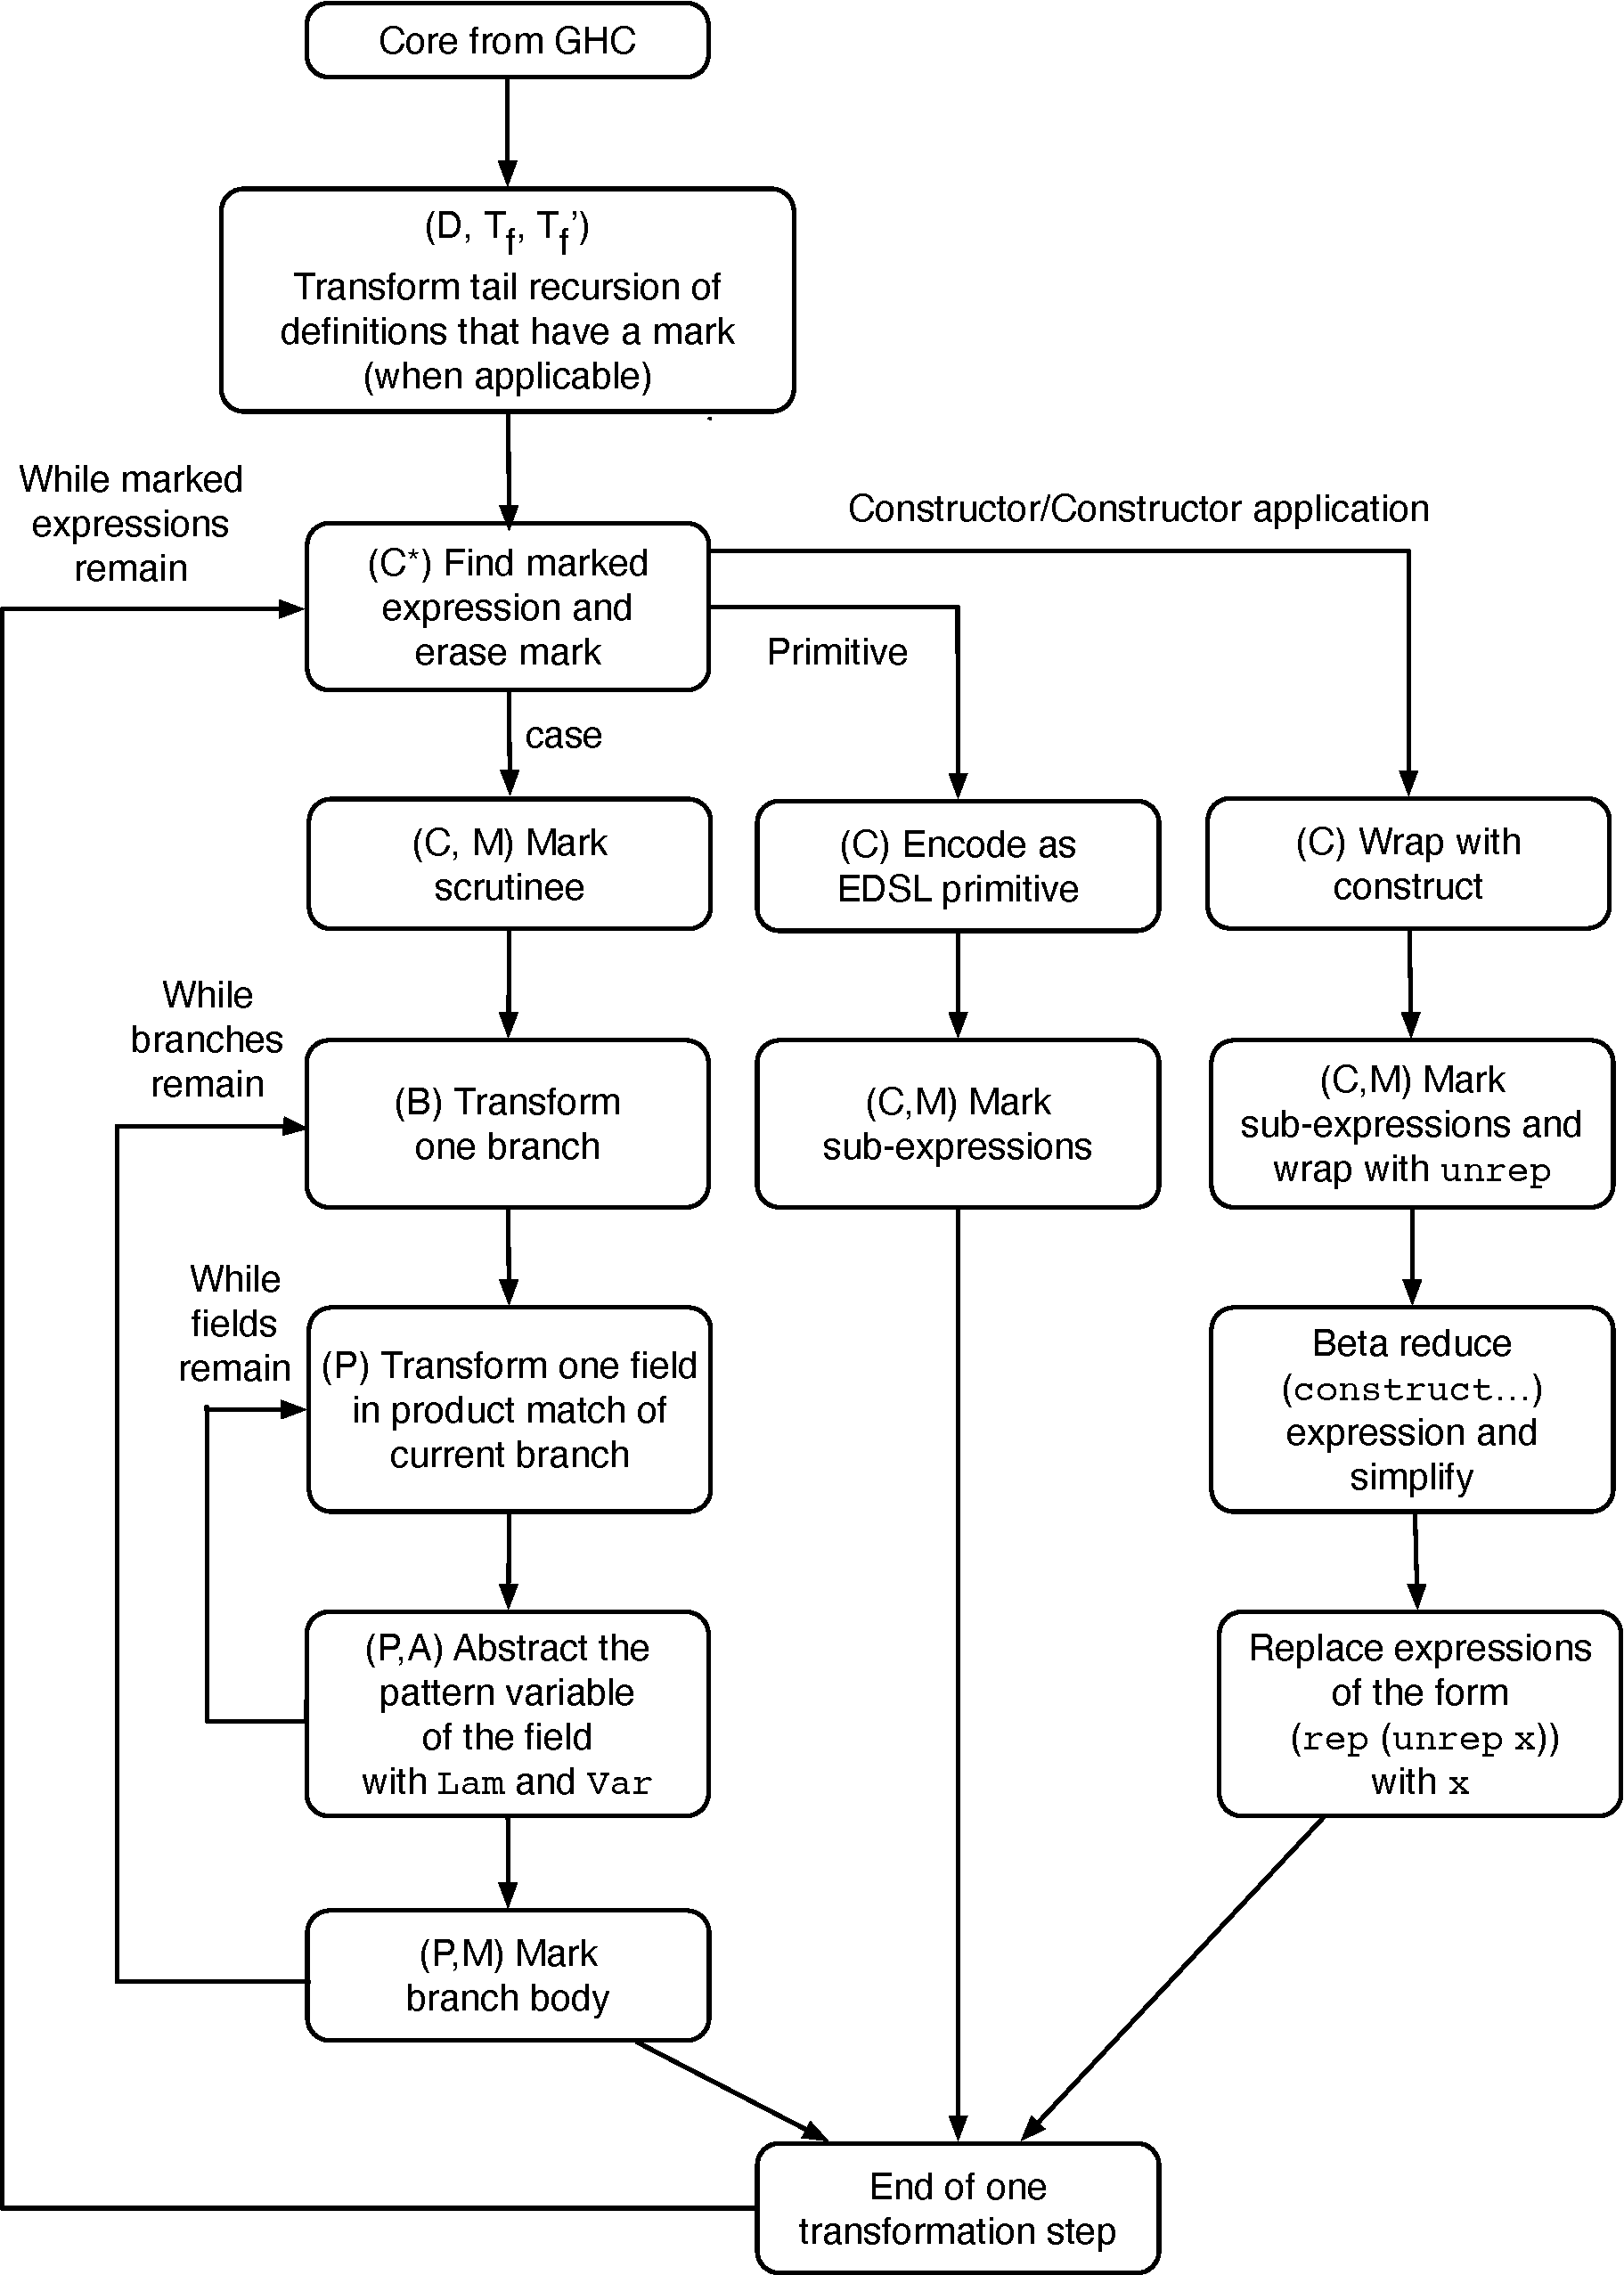
\includegraphics{Diagrams/Flowchart.pdf}}
   \caption{Control Flow of the Core Plugin}
   \label{fig:CorePlugin}
\end{figure*}

\clearpage

% \subsection{Syntactic Transformations of the Core Plugin}

% \begin{todo}
%   Should we use Oxford brackets here? Maybe a bit unusual, but we are operating syntactically and mapping from \ttt{a} to \ttt{E a} (could \ttt{E a} be considered an "intermediary" semantic domain?).
% \end{todo}
% \vspace*{-0.6cm}

\begin{figure*}[hp]
  \centering
\begin{align*}
  &D\expr{\ttt{f x = internalize (externalize (case s of \{ ... \}))}}
      \rewrites I(D(\ttt{f x = externalize (case s of \{ ... \})}))\\
  &D\expr{\ttt{f x = externalize (case s of \{ ... \})}}\\
      &\quad\rewrites \begin{cases}
        \ttt{f = $C^{*}\expr{\ttt{externalize ($\lambda \eta \rarr$ runIter ($\lambda \ttt{x} \rarr \ttt{case s of \{ $T'_{\ttt{f}}\exprdots$}$ \}) $\eta$)}}$} & \text{\parbox{5cm}{if \ttt{f} occurs free in \ttt{\{ ... \}}, where $\eta$ is a fresh name}}\\
        \\
        \ttt{f x = $C^{*}\expr{\ttt{externalize (case s of \{ ... \})}}$} & \text{otherwise}
      \end{cases}\\
  &\\
  &I\expr{\ttt{f x = externalize e}} \rewrites \ttt{f x = internalize (externalize e)}\\
  &I\expr{\ttt{f = externalize e}} \rewrites \ttt{f = internalize (externalize e)}\\
  &T'_{\ttt{f}}\expr{\ttt{K x0 ...$_U$ xN $\rarr$ case s of \{ ...$_V$ \}; ...$_W$}}\\
    &\quad\rewrites
        \ttt{K x0 ...$_U$ xN $\rarr$ $T_{\ttt{f}}\expr{\ttt{case s of \{ ...$_V$ \}}}$; $T'_{\ttt{f}}\expr{\ttt{ ...$_W$ }}$}\\
  &T'_{\ttt{f}}\expr{\ttt{K x0 ...$_U$ xN $\rarr$ body0; ...$_V$ }}\\
    &\quad\rewrites
      \begin{cases}
        \ttt{K x0 ...$_U$ xN $\rarr$ body0}[\ttt{f} \mapsto \ttt{Step}]\ttt{; }T'_{\ttt{f}}\expr{\ttt{ ...$_V$ }} & \text{if \ttt{f} occurs free in \ttt{body0}}\\
        \ttt{K x0 ...$_U$ xN $\rarr$ Done body0; $T'_{\ttt{f}}\expr{\ttt{ ...$_V$ }}$} & \text{otherwise}
      \end{cases}\\
  &T'_{\ttt{f}}\expr{\varepsilon} \rewrites \varepsilon\\
  &T_{\ttt{f}}\expr{\ttt{case s of \{ ... \}}}\\
    &\quad\rewrites
      \begin{cases}
        \ttt{case s of \{ $T'_{\ttt{f}}\expr{\ttt{ ... }}$ \}} & \text{if \ttt{f} occurs free in \ttt{\{ ... \}}}\\
        \ttt{Done (case s of \{ ... \})} & \text{otherwise}
      \end{cases}\\
  &C^{*}\expr{\ttt{x}} \rewrites
    \begin{cases}
      \ttt{x} & \text{if \ttt{x} has no subexpressions marked with \ttt{externalize}}\\
      C^{*}\expr{C\expr{\ttt{y}}} & \text{if \ttt{externalize y} is the first marked subexpression of \ttt{x}}\\
    \end{cases}\\
  &C\expr{\ttt{runIter f x}} \rewrites \ttt{App (TailRec $M\expr{\ttt{f}}$) $M\expr{\ttt{x}}$}\\
  &C\expr{\ttt{x + y}} \rewrites \ttt{Add $M\expr{\ttt{x}}$ $M\expr{\ttt{y}}$}\\
  &C\expr{\ttt{case scrutinee of \{ ... \}}} \rewrites \ttt{CaseExp $M\expr{\ttt{scrutinee}}$ } B\expr{\ttt{ ... }}\\
  &C\expr{\ttt{$\lambda$x $\rarr$ body}} \rewrites A\expr{\lambda \ttt{x} \rarr \ttt{body}}\\
  &C\expr{\ttt{K x0 ... xN }} \rewrites \ttt{construct (K (unrep $M\expr{\ttt{x0}}$) ... (unrep $M\expr{\ttt{xN}}$))}\;\;\;\;\text{(Where \ttt{K} is a constructor)}\\
  &C\expr{\ttt{f x}} \rewrites \ttt{App $M\expr{f}$ $M\expr{x}$}\\
  % &C\expr{\ttt{f x}} \rewrites \ttt{ConstructAp $M\expr{\ttt{f}}$ $M\expr{\ttt{x}}$}\;\;\;\;\text{(Where \ttt{f} is not a primitive or an application of a primitive)}\\
  % &C\expr{\ttt{x}} \rewrites \ttt{Construct x}\;\;\;\;\text{(Where \ttt{x} is a variable which is not a primitive)}\\
  &B\expr{\ttt{K x0 ...$_U$ xN $\rarr$ body0; ...$_V$}} \rewrites \ttt{SumMatchExp }P\expr{\ttt{x0 ...$_U$ xN $\rarr$ body0}}\; B\expr{\ttt{ ...$_V$ }}\\
  &B\expr{\ttt{K x0 ... xN $\rarr$ body}} \rewrites \ttt{OneSumMatchExp }P\expr{\ttt{x0 ... xN $\rarr$ body}}\\
  &B\expr{\ttt{$\varepsilon$}} \rewrites \ttt{EmptyMatch}\\
  &P\expr{\ttt{x0 x1 ... xN $\rarr$ body}} \rewrites \ttt{ProdMatchExp }A\expr{\ttt{$\lambda$ x0 $\rarr$ $P\expr{\ttt{x1 ... xN $\rarr$ body}}$}}\\
  &P\expr{\ttt{x $\rarr$ body}} \rewrites \ttt{OneProdMatchExp }A\expr{\ttt{$\lambda$ x $\rarr$ body}}\\
  &P\expr{\ttt{ $\rarr$ body}} \rewrites \ttt{NullaryMatch $M\expr{\ttt{body}}$}\\
  &A\expr{\ttt{$\lambda$(x :: a) $\rarr$ body}} \rewrites \ttt{Lam (Name @a uniq) $M\expr{\ttt{body$[\ttt{x} \mapsto \ttt{unrep (Var @a uniq)}]$}}$}\\
  &\text{\;\;\;\;\;(where \ttt{uniq} is a globally unique identifier)}\\
  &M\expr{\ttt{unrep x}} \rewrites \ttt{x}\\
  &M\expr{\ttt{x :: a}} \rewrites
    \begin{cases}
      \ttt{externalize x} & \text{if}\; \nexists t, a\; \typeeq E\; t\\
      \ttt{x} & \text{if}\; \exists t, a\; \typeeq E\; t
    \end{cases}
\end{align*}

\captionsetup{justification=centering}
\caption{Rewrite rules}
\label{fig:Rewrites}
\end{figure*}

% \clearpage

\clearpage
\section{Related Work}

% \begin{todo}
%   Does this need more fleshing out?
% \end{todo}

The basis of deep embeddings in functional languages is well understood.
\cite{Elliott:03:CompileDSEL-JFP} explains the basic idea, and \cite{Gill:2014:DSLSynth}
gives an acceessable and more recent account of the area.

A similar EDSL-oriented representation of pattern matching is given in
~\cite[Section~3.3]{Atkey:09:Unembedding}. In that paper, patterns were given their own
representation which allows for compound patterns. This is useful in the context
of that work, as the programmer works directly with these patterns.

In the present paper, however, the representation is generated automatically by
a compiler plugin. As a result of GHC's desugared Core (which does not have
compound patterns), there is no need to directly express compound patterns at
the representation-level.

There is other recent work using deep embeddings in functional languages for 
system development.  One example is the Ivory language \cite{Elliott2015-Ivory} 
which provides a deeply embedded DSL for use in programming high assurance
systems,  However, its syntax is typical of a deep EDSL and requires additional
keywords and structures above idiomatic Haskell. 

The Feldspar project~\cite{Axelsson:10:Feldspar,Svenningsson:13:Combining}
is a Haskell embedding of a monadic interface
that targets C, and focuses on high-performance.  Both Feldspar and our work
mix deep and shallow language constructs ~\cite{Persson:11:MonadicDSL,Svenningsson:13:Compositional,Sculthorpe:13:ConstrainedMonad}.

Svenningsson and Axelsson~\cite{Svenningsson:13:Combining}
explored combining deep and shallow embedding.  They used
a deep embedding as a low level language, then extended
the deep embedding with a shallow embedding written on top
of it. Haskell type classes were used to minimize the effort of adding
new features to the language.

Yin-Yang~\cite{Jovanovic:2014} provides a framework for DSL
embedding in Scala which uses Scala macros to provide the 
translation from a shallow to deep embedding.  Yin-Yang
goes beyond the translation by also providing autogeneration
of the deep DSL from the shallow DSL.  The focus of
Yin-Yang is in generalizing the shallow to deep transformations,
and does not include recursive transformations.

Forge~\cite{Sujeeth:2013} is a Scala based meta-EDSL framework
which can generate both shallow and deep embeddings from
a single EDSL specification.  Embeddings generated by Forge
use abstract \verb|Rep| types, analogous to our EDSL's 
\verb|E| types.  Their shallow embedding is generated
as a pure Scala library, while the deeply embedded version
is generated as an EDSL using the Delite~\cite{Sujeeth:2014}
framework.

Elliott developed GHC plugins~\cite{github:lambda-ccc}\cite{github:reification-rules}
for compiling Haskell to hardware~\cite{github:Elliott:Talk:2015},
using worker-wrapper style transformations~\cite{Gill:09:WW}
equivalent to the \verb|abs| and
\verb|rep| transformations described in Section~\ref{sec:Overview}. These plugins were later generalized to enable additional interpretations~\cite{Elliott:2017}.

% \section{Citations and Bibliographies}

\bibliographystyle{ACM-Reference-Format}
\bibliography{paper}

\appendix
\section{Additional Code for Standard Haskell Semantics Implementation}
\begin{lstlisting}[basicstyle=\tiny]
absEnv :: forall t. Env -> E t -> t
absEnv env (CaseExp x f) =
  sumMatchAbs f (absEnv env x)

absEnv env (TailRec f) = \ x ->
  case absEnv env f x of
    Step x' -> absEnv env (TailRec f) x'
    Done r  -> r

absEnv env (Var v) =
  case envLookup env v of
    Just x -> absEnv env
    Nothing ->
      error
        ("No binding for name "
          ++ show v)

absEnv env (Lam (name :: Name a)
                (body :: E b)) =
  \ (arg :: a) ->
    let go :: forall x. E x -> E x
        go expr@(Var name2 :: E a') =
          case namesEq name name2 of
            Just Refl -> rep arg
            _ ->
              case envLookup env name2 of
                Just v  -> v
                Nothing -> expr

        -- [... traverse rest of expression
        --      in go ...]
    in
    absEnv (extendEnv env
                      (name :=> rep arg))
           (go body)

absEnv env (LeftExp x) =
  Left (absEnv env x)

absEnv env (RightExp y) =
  Right (absEnv env y)

absEnv env (PairExp x y) =
  (absEnv env x, absEnv env y)

absEnv env (ConstructRep x) =
  unrep' (absEnv env x)

...
\end{lstlisting}

% \vfill\break

\section{A small EDSL for C code generation used internally by the C backend}
\begin{lstlisting}[basicstyle=\tiny]
type CCode = String
type CName = String

stmt :: CCode -> CCode
stmt = (<> ";")

cCall :: CName -> [CCode] -> CCode
cCall fnName args =
  fnName
  <> "(" <> intercalate ", " args <> ")"

derefPtr :: CCode -> CCode
derefPtr x = "*(" <> x <> ")"

cCast :: CCode -> CCode -> CCode
cCast toType x =
  "((" <> toType <> ")" <> x <> ")"

cIndex :: CCode -> Int -> CCode
cIndex x i =
  "(" <> x <> ")[" <> show i <> "]"

(!) :: CCode -> Int -> CCode
(!) = cIndex

(=:) :: CCode -> CCode -> CCode
x =: y = stmt (x <> " = " <> y)

cDecl :: CName -> CName -> CCode
cDecl cType v = stmt (cType <> " " <> v)

(#) :: CCode -> CName -> CCode
x # fieldName = x <> "." <> fieldName

macroDef
  :: CName -> [CName] -> [CCode]
     -> CCode
macroDef name args theLines =
  unlines
    [ "#define " <> name
              <> "(" <>
                intercalate ", " args
              <> ")\\"
    , "  do {\\"
    , unlines
        . map ("    "++)
        . map (++"\\")
        $ theLines
    , "  } while (0);"
    ]
\end{lstlisting}
% \begin{todo}
%   Fill in
% \end{todo}





% The use of \BibTeX\ for the preparation and formatting of one's
% references is strongly recommended. Authors' names should be complete
% --- use full first names (``Donald E. Knuth'') not initials
% (``D. E. Knuth'') --- and the salient identifying features of a
% reference should be included: title, year, volume, number, pages,
% article DOI, etc.

% The bibliography is included in your source document with these two
% commands, placed just before the \verb|\end{document}| command:
% \begin{verbatim}
%   \bibliographystyle{ACM-Reference-Format}
%   \bibliography{bibfile}
% \end{verbatim}
% where ``\verb|bibfile|'' is the name, without the ``\verb|.bib|''
% suffix, of the \BibTeX\ file.

% Citations and references are numbered by default. A small number of
% ACM publications have citations and references formatted in the
% ``author year'' style; for these exceptions, please include this
% command in the {\bfseries preamble} (before
% ``\verb|\begin{document}|'') of your \LaTeX\ source:
% \begin{verbatim}
%   \citestyle{acmauthoryear}
% \end{verbatim}

%   Some examples.  A paginated journal article \cite{Abril07}, an
%   enumerated journal article \cite{Cohen07}, a reference to an entire
%   issue \cite{JCohen96}, a monograph (whole book) \cite{Kosiur01}, a
%   monograph/whole book in a series (see 2a in spec. document)
%   \cite{Harel79}, a divisible-book such as an anthology or compilation
%   \cite{Editor00} followed by the same example, however we only output
%   the series if the volume number is given \cite{Editor00a} (so
%   Editor00a's series should NOT be present since it has no vol. no.),
%   a chapter in a divisible book \cite{Spector90}, a chapter in a
%   divisible book in a series \cite{Douglass98}, a multi-volume work as
%   book \cite{Knuth97}, an article in a proceedings (of a conference,
%   symposium, workshop for example) (paginated proceedings article)
%   \cite{Andler79}, a proceedings article with all possible elements
%   \cite{Smith10}, an example of an enumerated proceedings article
%   \cite{VanGundy07}, an informally published work \cite{Harel78}, a
%   doctoral dissertation \cite{Clarkson85}, a master's thesis:
%   \cite{anisi03}, an online document / world wide web resource
%   \cite{Thornburg01, Ablamowicz07, Poker06}, a video game (Case 1)
%   \cite{Obama08} and (Case 2) \cite{Novak03} and \cite{Lee05} and
%   (Case 3) a patent \cite{JoeScientist001}, work accepted for
%   publication \cite{rous08}, 'YYYYb'-test for prolific author
%   \cite{SaeediMEJ10} and \cite{SaeediJETC10}. Other cites might
%   contain 'duplicate' DOI and URLs (some SIAM articles)
%   \cite{Kirschmer:2010:AEI:1958016.1958018}. Boris / Barbara Beeton:
%   multi-volume works as books \cite{MR781536} and \cite{MR781537}. A
%   couple of citations with DOIs:
%   \cite{2004:ITE:1009386.1010128,Kirschmer:2010:AEI:1958016.1958018}. Online
%   citations: \cite{TUGInstmem, Thornburg01, CTANacmart}. Artifacts:
%   \cite{R} and \cite{UMassCitations}.

% \section{Acknowledgments}

%Identification of funding sources and other support, and thanks to
%individuals and groups that assisted in the research and the
%preparation of the work should be included in an acknowledgment
%section, which is placed just before the reference section in your
%document.

%This section has a special environment:
%\begin{verbatim}
%  \begin{acks}
%  ...
%  \end{acks}
%\end{verbatim}
%so that the information contained therein can be more easily collected
%during the article metadata extraction phase, and to ensure
%consistency in the spelling of the section heading.

%Authors should not prepare this section as a numbered or unnumbered {\verb|\section|}; please use the ``{\verb|acks|}'' environment.

%\section{Appendices}

%If your work needs an appendix, add it before the
%``\verb|\end{document}|'' command at the conclusion of your source
%document.

%Start the appendix with the ``\verb|appendix|'' command:
%\begin{verbatim}
%  \appendix
%\end{verbatim}
%and note that in the appendix, sections are lettered, not
%numbered. This document has two appendices, demonstrating the section
%and subsection identification method.

%\section{SIGCHI Extended Abstracts}

%The ``\verb|sigchi-a|'' template style (available only in \LaTeX\ and
%not in Word) produces a landscape-orientation formatted article, with
%a wide left margin. Three environments are available for use with the
%``\verb|sigchi-a|'' template style, and produce formatted output in
%the margin:
%\begin{itemize}
%\item {\verb|sidebar|}:  Place formatted text in the margin.
%\item {\verb|marginfigure|}: Place a figure in the margin.
%\item {\verb|margintable|}: Place a table in the margin.
%\end{itemize}

%%%
%%% The acknowledgments section is defined using the "acks" environment
%%% (and NOT an unnumbered section). This ensures the proper
%%% identification of the section in the article metadata, and the
%%% consistent spelling of the heading.
%\begin{acks}
%To Robert, for the bagels and explaining CMYK and color spaces.
%\end{acks}

%%%
%%% The next two lines define the bibliography style to be used, and
%%% the bibliography file.
%\bibliographystyle{ACM-Reference-Format}
%\bibliography{sample-base}

%%%
%%% If your work has an appendix, this is the place to put it.
%\appendix

%\section{Research Methods}

%\subsection{Part One}

%Lorem ipsum dolor sit amet, consectetur adipiscing elit. Morbi
%malesuada, quam in pulvinar varius, metus nunc fermentum urna, id
%sollicitudin purus odio sit amet enim. Aliquam ullamcorper eu ipsum
%vel mollis. Curabitur quis dictum nisl. Phasellus vel semper risus, et
%lacinia dolor. Integer ultricies commodo sem nec semper.

%\subsection{Part Two}

%Etiam commodo feugiat nisl pulvinar pellentesque. Etiam auctor sodales
%ligula, non varius nibh pulvinar semper. Suspendisse nec lectus non
%ipsum convallis congue hendrerit vitae sapien. Donec at laoreet
%eros. Vivamus non purus placerat, scelerisque diam eu, cursus
%ante. Etiam aliquam tortor auctor efficitur mattis.

%\section{Online Resources}

%Nam id fermentum dui. Suspendisse sagittis tortor a nulla mollis, in
%pulvinar ex pretium. Sed interdum orci quis metus euismod, et sagittis
%enim maximus. Vestibulum gravida massa ut felis suscipit
%congue. Quisque mattis elit a risus ultrices commodo venenatis eget
%dui. Etiam sagittis eleifend elementum.

%Nam interdum magna at lectus dignissim, ac dignissim lorem
%rhoncus. Maecenas eu arcu ac neque placerat aliquam. Nunc pulvinar
%massa et mattis lacinia.

\end{document}
\endinput
